\section{Modeling Automotive Systems}
\label{model_automotive_sys}
In this chapter, we will discuss a number of simplified mathematical models that can be used to model various aspects
of an automobile. Concretely, we will cover the follwoing:

\begin{itemize}
\item Longitudinal vehicle dynamics
\item Drivetrain modeling
\item Suspension modeling
\item Single track model
\end{itemize}

In doing so, we will present and apply a three phase modeling method that comprises of three steps. Namely,

\begin{itemize}
\item Structuring
\item Constitutive relationships
\item State-space model formulation
\end{itemize}
 

\section{Longitudinal Dynamics}
\label{longitudinal_dynamics}
In this section we are interested in developing a model that captures the main longitudinal dynamics of the vehicle. Concretely, we are interested in
how the velocity of the vehicle changes when we press or release the accelerator pedal. We will follow the three phase modeling approach. 

\subsection{Structuring}
Let's assume that the vehicle consists of the powertrain and the chassis. The former produces a propulsion force $\mathbf{F}_p$ that acts on the latter. We can visualize this 
using a block diagram as shown in figure \ref{powertrain_chassis}:

\begin{figure}[!htb]
\begin{center}
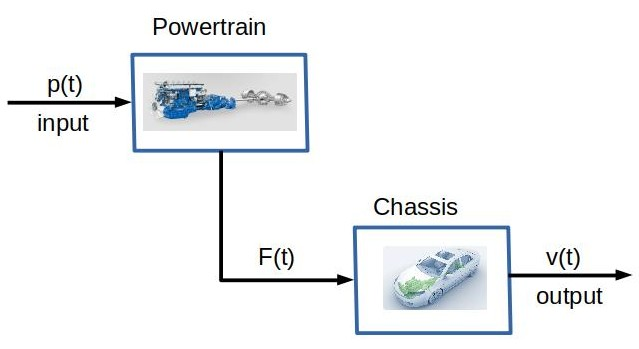
\includegraphics[scale=0.280]{img/model_automotive_sys/powertrain_chassis.jpg}
\end{center}
\caption{Block diagram for powertrain-chassis relationship.}
\label{powertrain_chassis}
\end{figure}

The powertrain can be further broken down into several other subsystems such as:

\begin{itemize}
\item Engine
\item Gearbox
\item Wheels
\end{itemize}

This is shown in the block diagram in figure \ref{engine_gearbox_wheel_block_diagram}


\begin{figure}[!htb]
\begin{center}
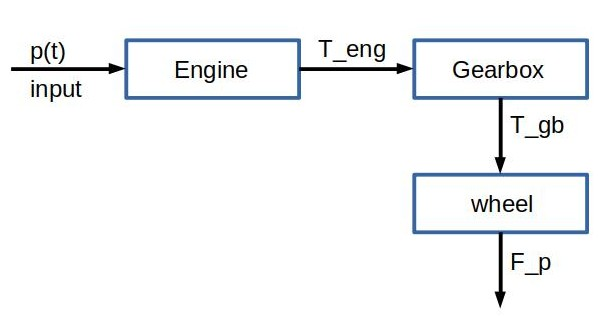
\includegraphics[scale=0.280]{img/model_automotive_sys/engine_gearbox_wheel_block_diagram.jpg}
\end{center}
\caption{Block diagram for engine-gearbox-wheels relationship.}
\label{engine_gearbox_wheel_block_diagram}
\end{figure}



The advantage of such fine grained approach is that we can describe the various components individually. However, the downside is that we increase
the complexity of our model. Hopefully, this increase in complexity will be reflected in an increase of  accuracy of the resulting model.

Let's now start modeling the powertrain. 

\subsection{Powertrain Modeling}

By pressing the pedal, the engine responds by building up a torque $T_{eng}$. We will assume that this build up process can be adequately represented by a first
order dynamics. Thus,

\begin{equation}
\dot{T}_{eng } = - \frac{1}{\tau}T_{eng} + \frac{k}{\tau} p 
\label{engine_model}
\end{equation}

where

\begin{itemize}
\item $p$ is the pedal position
\item $k$ is the steady state gain from the pedal position
\item $\tau$ is the time constant of the engine to build up the torque
\end{itemize}


The gearbox will simply amplify the engine torque, $T_{eng}$,  with a factor equal to the gear ratio $i$ as given by the equation below

\begin{equation}
T_{gb } = iT_{eng} 
\label{gear_model} 
\end{equation}



The wheels convert the torque to force via the wheel radius $r_w$ 

\begin{equation}
\mathbf{F} = \frac{T_{gb}}{r_w}  
\label{wheel_model}
\end{equation}

The wheel model in equation \ref{wheel_model} assumes that there is no slip between the wheels and the ground. 

If we substitute the models \ref{wheel_model} and \ref{gear_model} into \ref{engine_model}, we obtain the following equation for $\mathbf{F}$ which from now on we will call the propulsion force and indicate it instead with $\mathbf{F}_p$


\begin{equation}
\frac{d\mathbf{F}_p}{dt} = - \frac{1}{\tau}\mathbf{F}_p + \frac{ki}{\tau r_w} p   
\label{engine_model_II}
\end{equation}

\subsection{Chassis Modeling}
The propulsion force, $\mathbf{F}_p$, produced by the powertrain can be given as an input to the chassis model as shown schematically in figure

 
\begin{figure}[!htb]
\begin{center}
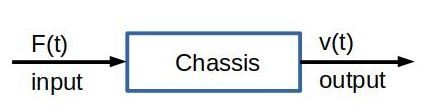
\includegraphics[scale=0.280]{img/model_automotive_sys/chassis_block_diagram.jpg}
\end{center}
\caption{Block diagram for chassis component.}
\label{chassis_block_diagram}
\end{figure}

We can derive the governing equation describing the dynamics of the chassis by using Newton's law:

\begin{equation}
m\mathbf{a} =  \mathbf{F}_T 
\label{chassis_force_balance}
\end{equation}

where $m$ is the vehicle mass and $\mathbf{F}_T$ is the total or net force acting on the chassis. The net force is assumed to have the following components 

\begin{itemize}
\item $\mathbf{F}_p$ propulsion force
\item $\mathbf{F}_{aero}$ aerodynamic force coming from the movement of the vehicle
\item $\mathbf{F}_{grav}$ the graviational force
\item $\mathbf{F}_{roll}$ the rolling resistance force
\end{itemize}

Thus,

\begin{equation}
\mathbf{F}_T = \sum_{i} \mathbf{F}_i =  \mathbf{F}_p -  \mathbf{F}_{aero} - \mathbf{F}_{grav} -  \mathbf{F}_{roll}
\label{chassis_model_total_force}
\end{equation}

The propulsion force is assumed to act in the direction of motion and must be large enough to overcome the three other forces in order for
the vehicle to able to move. The following body diagram illustrates this.


\begin{figure}[!htb]
\begin{center}
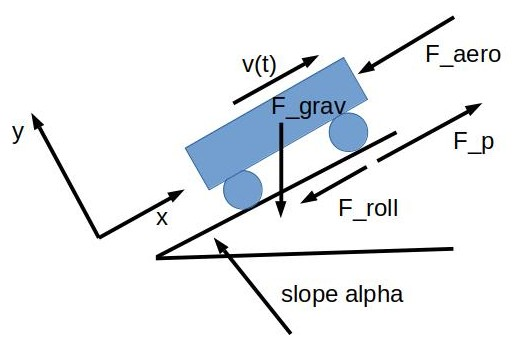
\includegraphics[scale=0.280]{img/model_automotive_sys/free_diagram_chassis.jpg}
\end{center}
\caption{Chassis free body diagram.}
\label{free_diagram_chassis}
\end{figure}

Note that in the figure above the propulsion and rolling forces are only shown to act in one wheel which is not true.

Since we assume that the road has slope $\alpha$,  it useful to decompose the forces in the $x$ and $y$ direction:


\begin{eqnarray}
x: m\alpha_x = F_{p, x} - F_{aero,x} - F_{grav, x} - F_{roll, x}  \\
y: m\alpha_y = F_{p, y} - F_{aero,y} - F_{grav, y} - F_{roll, y}  \\
\label{chassis_model_force_decomp}
\end{eqnarray}


\subsection{Balance Laws \& Constitutive Equations}

Let's now turn attention to the constitutive equations. Ideally, we would not like to have any accelerations in the $y$ direction thus $\alpha_y =0$. Furthermore, there in no drag force component
in the in the $y$ direction; $F_{aero,y} = 0$ whilst the drag term in the $x$ direction is modelled via:

\begin{equation}
F_{aero,x} = \frac{1}{2}\rho C_D A_f v^2 
\label{chassis_model_drag_term}
\end{equation}

where

\begin{itemize}
\item $\rho$ is the air density
\item $C_D$ is the drag coefficient
\item $\mathbf{F}_{grav}$ the graviational force
\item $\mathbf{F}_{roll}$ the rolling resistance force
\end{itemize}

From figure \ref{gravity_decomp_diagram}


\begin{figure}[!htb]
\begin{center}
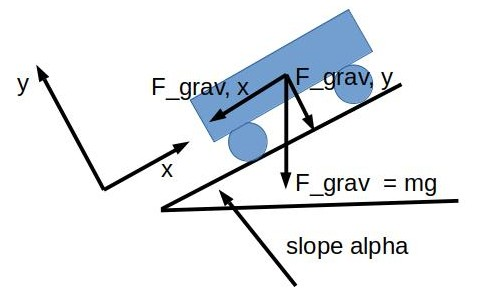
\includegraphics[scale=0.280]{img/model_automotive_sys/gravity_decomp_diagram.jpg}
\end{center}
\caption{$\mathbf{F}_{grav}$ force decomposition.}
\label{gravity_decomp_diagram}
\end{figure}


we can decompose the $\mathbf{F}_{grav}$ into 

\begin{eqnarray}
x: F_{grav, x} = mg\sin(\alpha)  \\
y: F_{grav, y} = mg\cos(\alpha) 
\label{gravity_decomp}
\end{eqnarray}

Finally, the rolling force in the x-direction $F_{roll, x}$ is modelled as a fraction of the vehicle load:

\begin{equation}
F_{roll,x} = (N_1 + N_2)f
\label{chassis_model_roll_force}
\end{equation}


\subsection{Summary Of Balance Laws \& Constitutive Equations}
Let's now summarize the equations and constitutive relations used for our model. Note that the acceleration $\boldsymbol{\alpha}$  is given by

\begin{eqnarray}
\boldsymbol{\alpha} = \frac{d \mathbf{v}}{dt}
\label{acceleration_vel_relationship}
\end{eqnarray}

\begin{itemize}
\item Chassis dynamics 
\end{itemize}

\begin{eqnarray}
x: m\alpha_x = F_{p, x} - F_{aero,x} - F_{grav, x} - F_{roll,x}  \\
y: 0 = N_1 + N_2 - F_{grav, y} 
\label{chassis_model_summary}
\end{eqnarray}

where

\begin{itemize}
\item $F_{aero,x} = \frac{1}{2}\rho C_D A_f v^2 $ 
\item $F_{grav, x} = mg \sin(\alpha)$ 
\item $F_{grav, y} = mg \cos(\alpha)$ 
\item $F_{roll,x} = (N_1 + N_2)f$ the graviational force
\item $N_1,  N_2$ are the vehicle load on the back and front wheels respectively 
\end{itemize}

The propulsion force $\mathbf{F}_p$ is given by the solution of

\begin{equation}
\frac{d\mathbf{F}_p}{dt} = - \frac{1}{\tau}\mathbf{F}_p + \frac{ki}{\tau r_w} p   
\label{engine_model_III}
\end{equation}


\subsection{State-Space Form}
We will now cast the model above into the state-space form. The first step is to select the state variables. We do so by observing what changes. We have two items here

\begin{itemize}
\item The propulsion force $\mathbf{F}_p$  
\item The velocity $\mathbf{v}$
\end{itemize}


\section{Questions}

\textbf{Question 1}

Consider the the longitudinal motion vehicle model

\begin{eqnarray}
\frac{dx_1}{dt} = \frac{1}{\tau}x_1 + \frac{ki}{\tau r_w} u \nonumber \\
\frac{dx_2}{dt} = \frac{1}{m} \left ( x_1 - mgf\cos(\alpha) - \frac{1}{2}\rho C_DA_f x_{2}^2 - mg\sin(\alpha) \right )  \nonumber \\
y = x_2 \nonumber
\end{eqnarray}

where  $x-1$ is the force at the wheels, $x_2$ is the vehicle velocity, $u$ is the input signal, the accelerator pedal position, and $\alpha$ is the disturbance, the road slope.

Is the longitudinal vehicle dynamics model linear?

Is the longitudinal vehicle dynamics model time invariant?

Determine the required engine torque (Nm) for a vehicle acceleration of 0.3 $m/s^2$ on a flat road at 60 $km/h$!


Longitudinal slip is the relative motion between a tire and the road surface it is moving on: 

\begin{equation}
\text{slip} = \frac{r_w \omega - v}{v}
\end{equation}

which means that the wheels are spinning if slip is positive and that the wheels are skidding if slip is negative. The longitudinal vehicle dynamics model is developed under the assumption that the relative motion between the tire and the road surface is zero, i.e. is not included in the model.

If we would like to include slip into our model, how many additional states are needed in order to include longitudinal slip into the model?


One additional state is needed as we need to include the wheel speed as an additional state variable in order to capture slip as we already have velocity as one state. 

When performing numerical simulations with the longitudinal vehicle dynamics model including the slip model, you might run into numerical problems. Why?

\begin{itemize}
\item A) Division by zero, due to zero velocity 
\item B) Division by zero, due to zero wheel speed 
\item C) Division by zero, due to zero engine torque 
\end{itemize}

The slip model includes a normalization with respect to the vehicle velocity. This gives numerical problems when the velocity is zero, i.e. division by zero. Thus, option A is the correct answer.


\section{Drivetrain Modeling}

\section{Suspension System Modeling}

In this section we will derive a mathematical model for the vehicle suspension system. Concretely, we will assume a passive suspension system.


\begin{framed}

\textbf{Active and Passive Suspension System}

Active suspension is a type of automotive suspension that controls the vertical movement of the wheels relative to the chassis or vehicle body with an onboard system, rather than in passive suspension where the movement is being determined entirely by the road surface. Active suspensions can be generally divided into two classes: 

\begin{itemize}
\item pure active suspensions, 
\item adaptive/semi-active suspensions. 
\end{itemize}
While adaptive suspensions only vary shock absorber firmness to match changing road or dynamic conditions, active suspensions use some type of actuator to raise and lower the chassis independently at each wheel. For more information see the Wikipedia entry: https://en.wikipedia.org/wiki/Active\_suspension

\end{framed}


The suspension system connects the vehicle body with the wheels. furthermore, it gives the whell a vertical movement possibility. A common approach to model the vehicle suspension
system is to consider only one of the four wheels. The schematic of a simplified suspension system is shown in figure

For a passive suspension system, the input is road surface $z_r$. The outputs will be the positions of the wheels $z_w$ and that of the chassis $z_c$. The block diagram is shown in figure
\ref{suspension_sys_block_diagram} 

\begin{figure}[!htb]
\begin{center}
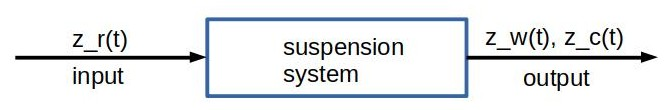
\includegraphics[scale=0.280]{img/model_automotive_sys/suspension_sys_block_diagram.jpg}
\end{center}
\caption{Block diagram for suspension system.}
\label{suspension_sys_block_diagram}
\end{figure}

The free body diagram for the wheel mass is shown in figure \ref{suspension_sys_wheel_mass_free_diagram}


\begin{figure}[!htb]
\begin{center}
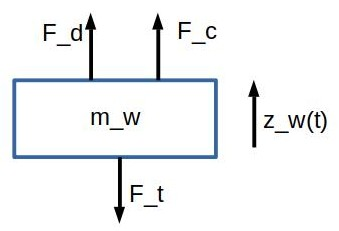
\includegraphics[scale=0.280]{img/model_automotive_sys/suspension_sys_wheel_mass_free_diagram.jpg}
\end{center}
\caption{Wheel mass free body diagram.}
\label{suspension_sys_wheel_mass_free_diagram}
\end{figure}

where $\mathbf{F}_t$ is the tire force, $\mathbf{F}_d$ is the suspension force and $\mathbf{F}_c$ is the chassis force. Similarly, the free body diagram for the chassis mass is shown in figure \ref{suspension_sys_wheel_mass_free_diagram}

\begin{figure}[!htb]
\begin{center}
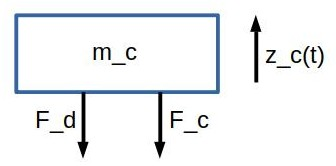
\includegraphics[scale=0.280]{img/model_automotive_sys/suspension_sys_chassis_mass_free_diagram.jpg}
\end{center}
\caption{Chassis mass free body diagram.}
\label{suspension_sys_chassis_mass_free_diagram}
\end{figure}


\section{The Bicycle Model}
\label{bicycle_model}

We would like to be able to control the vehicle; for example when following a predefined path or when making an avoidance manouver. These types of motions
require control of the lateral dynamics that the longitudinal model developed in section \ref{longitudinal_dynamics} does not account for. We would like therefore
to generalize somehow our model.

Thus, in  this  section,  we  study the kinematic bicycle model, which is often used for trajectory planning,  
and  compare  its  results  to  a  none  degrees  of  freedom model. Modeling errors and limitations of the kinematic bicycle model are highlighted. 

The three degrees of freedoom (DOFs) kinematic bicycle model, see figure \ref{bicycle_model_1},  is one
of the simplest models frequently used at the motion planning phase, with the belief that it is able to capture enough of the
nonholonomic constraints of the actual vehicle dynamics. By constrast, even relatively simple vehicle models used for low level  control  can  imply  more  
than  ten DOFs \cite{Polack2017}. 


\begin{figure}[!htb]
\begin{center}
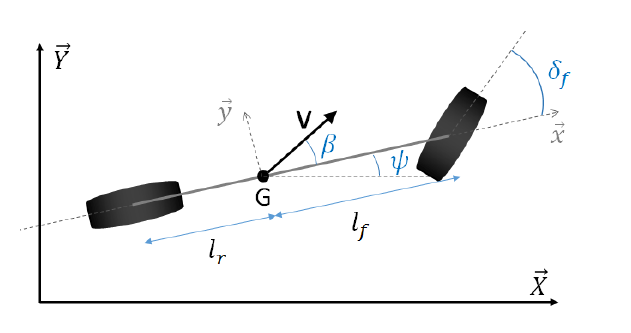
\includegraphics[scale=0.290]{img/model_automotive_sys/bicycle_model_1.jpeg}
\end{center}
\caption{Schematic of the bicycle model.}
\label{bicycle_model_1}
\end{figure}


In the kinematic bicycle model, the two front wheels (respectively the two rear wheels) of the vehicle are lumped into a unique
wheel  located  at  the  center  of  the  front  axle  (respectively  of  the rear axle) such as illustrated on Figure 1. 
The control inputs correspond to the acceleration $\boldsymbol{\alpha}$ and the front wheel steering angle $\delta$
of  the  vehicle,  when  assuming  that  only  the  front wheel can be steered. The kinematic bicycle model can then


